\documentclass{beamer}
\mode<presentation>
\usepackage{amsmath,amssymb,mathtools}
\usepackage{textcomp}
\usepackage{gensymb}
\usepackage{adjustbox}
\usepackage{subcaption}
\usepackage{enumitem}
\usepackage{multicol}
\usepackage{listings}
\usepackage{url}
\usepackage{graphicx} % <-- needed for images
\def\UrlBreaks{\do\/\do-}

\usetheme{Boadilla}
\usecolortheme{lily}
\setbeamertemplate{footline}{
  \leavevmode%
  \hbox{%
  \begin{beamercolorbox}[wd=\paperwidth,ht=2ex,dp=1ex,right]{author in head/foot}%
    \insertframenumber{} / \inserttotalframenumber\hspace*{2ex}
  \end{beamercolorbox}}%
  \vskip0pt%
}
\setbeamertemplate{navigation symbols}{}

\lstset{
  frame=single,
  breaklines=true,
  columns=fullflexible,
  basicstyle=\ttfamily\tiny   % tiny font so code fits
}

\numberwithin{equation}{section}

% ---- your macros ----
\providecommand{\nCr}[2]{\,^{#1}C_{#2}}
\providecommand{\nPr}[2]{\,^{#1}P_{#2}}
\providecommand{\mbf}{\mathbf}
\providecommand{\pr}[1]{\ensuremath{\Pr\left(#1\right)}}
\providecommand{\qfunc}[1]{\ensuremath{Q\left(#1\right)}}
\providecommand{\sbrak}[1]{\ensuremath{{}\left[#1\right]}}
\providecommand{\lsbrak}[1]{\ensuremath{{}\left[#1\right.}}
\providecommand{\rsbrak}[1]{\ensuremath{\left.#1\right]}}
\providecommand{\brak}[1]{\ensuremath{\left(#1\right)}}
\providecommand{\lbrak}[1]{\ensuremath{\left(#1\right.}}
\providecommand{\rbrak}[1]{\ensuremath{\left.#1\right)}}
\providecommand{\cbrak}[1]{\ensuremath{\left\{#1\right\}}}
\providecommand{\lcbrak}[1]{\ensuremath{\left\{#1\right.}}
\providecommand{\rcbrak}[1]{\ensuremath{\left.#1\right\}}}
\theoremstyle{remark}
\newtheorem{rem}{Remark}
\newcommand{\sgn}{\mathop{\mathrm{sgn}}}
\providecommand{\abs}[1]{\left\vert#1\right\vert}
\providecommand{\res}[1]{\Res\displaylimits_{#1}}
\providecommand{\norm}[1]{\lVert#1\rVert}
\providecommand{\mtx}[1]{\mathbf{#1}}
\providecommand{\mean}[1]{E\left[ #1 \right]}
\providecommand{\fourier}{\overset{\mathcal{F}}{ \rightleftharpoons}}
\providecommand{\system}{\overset{\mathcal{H}}{ \longleftrightarrow}}
\providecommand{\dec}[2]{\ensuremath{\overset{#1}{\underset{#2}{\gtrless}}}}
\newcommand{\myvec}[1]{\ensuremath{\begin{pmatrix}#1\end{pmatrix}}}
\newcommand{\mydet}[1]{\ensuremath{\begin{vmatrix}#1\end{vmatrix}}}

\newenvironment{amatrix}[1]{%
  \left(\begin{array}{@{}*{#1}{c}|*{#1}{c}@{}}
}{%
  \end{array}\right)
}

\newcommand{\myaugvec}[2]{\ensuremath{\begin{amatrix}{#1}#2\end{amatrix}}}
\let\vec\mathbf
% ---------------------

\title{Matgeo Presentation - Problem 12.381}
\author{ee25btech11056 - Suraj.N}

\begin{document}

\begin{frame}
  \titlepage
\end{frame}

\begin{frame}{Problem Statement}

Consider the matrix

\begin{align*}
\vec{A} = \myvec{4 & 0 \\ 0 & 4}
\end{align*}
Which one of the following vectors is \textbf{NOT} a valid eigenvector of the above matrix?

\begin{itemize}
\begin{multicols}{4}
\item $\myvec{1\\0}$
\item $\myvec{-2\\1}$
\item $\myvec{4\\-3}$
\item $\myvec{0\\0}$
\end{multicols}
\end{itemize}

\end{frame}

\begin{frame}{Data}

\begin{table}[h!]
  \centering
  \begin{tabular}{|c|c|}
\hline
\textbf{Name} & \textbf{Value} \\ \hline
$\vec{A}$ & $\myvec{2 & 1 \\0 & 3}$ \\ \hline
\end{tabular}

  \caption*{Table : Matrix}
  \label{12.381}
\end{table}

\end{frame}

\begin{frame}{Solution}

Since $\vec{A}$ is diagonal, its eigenvalues are the diagonal entries.

\begin{align}
\lambda_1 = 4,\quad \lambda_2 = 4
\end{align}

To find eigenvectors, we solve:

\begin{align}
  (\vec{A}-\lambda\vec{I})\vec{v} = \vec{0}
\end{align}

For $\lambda = 4$:

\begin{align}
  \vec{A}-4\vec{I} &= \myvec{4 & 0 \\ 0 & 4} - \myvec{4 & 0 \\ 0 & 4} \\
&= \myvec{0 & 0 \\ 0 & 0}
\end{align}

\end{frame}

\begin{frame}{Solution}

So:

\begin{align}
  (\vec{A}-4\vec{I})\vec{v} = \myvec{0 & 0 \\ 0 & 0}\vec{v} = \vec{0}
\end{align}

Thus, every $\vec{v} \in \mathbb{R}^2$ satisfies this equation.  
But an eigenvector must be nonzero.  \\

\textbf{Conclusion:} Any nonzero vector is an eigenvector corresponding to $\lambda=4$.  
The zero vector $\myvec{0\\0}$ is \textbf{not} a valid eigenvector.

\end{frame}

\begin{frame}{Plot}

\begin{figure}[h!]
  \centering
  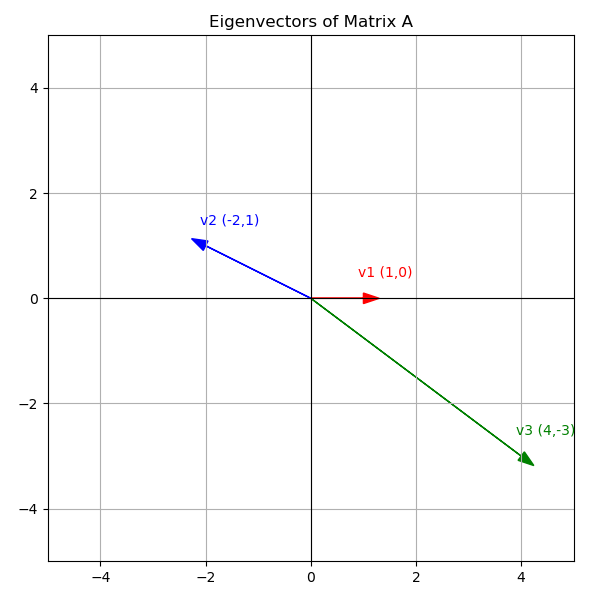
\includegraphics[width=0.6\columnwidth]{figs/eigenvectors.png} 
   \caption*{Fig : Eigen Vectors}
  \label{Fig1}
\end{figure}

\end{frame}

\end{document}



